\documentclass[a4paper, 10pt]{article}
\usepackage[utf8x]{inputenc}
\usepackage{graphicx}
\usepackage{geometry}
\usepackage{amsmath}
\usepackage{mathenv}
\usepackage{amssymb}
\usepackage{amsfonts}
\usepackage{mathrsfs}
\usepackage{textcomp}
\geometry{hmargin = 2.5cm, vmargin = 1.5cm}

% OPENING
\title{SY19 - TP01\\Positionnement multidimensionnel}
\author{Bertrand Bon - Antoine Hars}

\begin{document}

\maketitle

\section*{Exercice 1 : Exercice théorique}
On considère le tableau de données suivant :\\ \\
X = $\begin{pmatrix} 8.5 & 1.5 \\ 3.5 & 5.0 \\ 2.0 & 6.5 \\ 9.5 & 1.5 \\ 8.5 & 2.5 \\ 3.0 & 6.5 \\ 9.0 & 2.5 \\ 2.0 & 5.5 \end{pmatrix}$\\ \\
Dans cet exercice, nous avons étudié l'analyse en composantes principales (ACP) de cette matrice (variables quantitatives).\\
Pour ce faire, nous avons tout d'abord, centré la matrice X, puis nous avons calculé

\section*{Exercice 3 : Les données de distances entre aéroports}
Dans cet exercice, nous avons travaillé sur les données contenues dans le fichier \textit{airport2.txt} qui représentent les distances de vol
entre des aéroports situés dans le monde. L'objectif de cet exercice était d'appliquer les différentes méthodes
de positionnement multidimensionnel à ces données et de comparer les résultats obtenus.\\ \\
% Question 1
\textbf{Réalisation de l'AFTD sur les données avec \textit{cmdscale} et analyse des résultats obtenus.}\\
L'exécution de la fonction \textit{cmdscale} sur le tableau de distance des données nous a donné le graphique suivant :\\
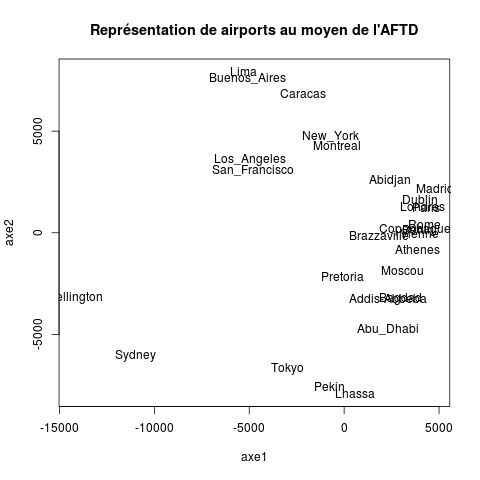
\includegraphics[height = 8cm, width = 8cm]{plots/plot_airports_cmdscale.png}\\

\end{document}
